\chapter{Model Description, Data and Analysis Method} 
In this thesis, the dust emission model 
FLEXDUST\footnote{\url{https://git.nilu.no/christine/flexdust/-/tree/a1ed0db98f345e1b56b570641d4871d22908a194} (last access 23/07/2021)} 
\parencite{flexdust_ref_2016} and the Lagrangian particle dispersion model 
FLEXPART\footnote{ \url{https://git.nilu.no/flexpart/flexpart/-/tree/release-10.4.1} (last access 06/05/2021)} 
\parencite{Flexpart10.4_ref} was used to 
simulate the spring time dust deposition between 1999 and 2019 at 7 sites across the Chinese Loess Plateau. Both FLEXDUST and FLEXPART are developed at the Norwegian Institute for air research (NILU). A copy of the exact source code can also be downloaded here \url{10.5281/zenodo.5128338}. 

\textcite{flexdust_ref_2016} used the same two models to study the transport and deposition of high latitude dust, where they simulated the dust transport from a source-oriented viewpoint, following the dust from the source to deposition. 
Here, the dust transport and deposition are simulated from a receptor viewpoint. 
All the dust deposited at the receptor location is tracked backwards in time to probe for possible sources. 
The emission field produced by FLEXDUST then constrains the distribution of possible the sources regions. 
The flow chart in \Cref{fig: flow_chart} summarises the modelling workflow. The receptor oriented backward approach was chosen over the forward approach due to being more computationally efficient when the number of source elements greatly exceeds the number of receptors. 
In addition, the backward approach allows for dealing with point receptors naturally. 
% In a forward simulation, the deposition at the receptor location must be interpolated from the model output grid. 
The backward approach also makes it possible to determine exact the source regions that contribute to deposition at the receptor. 

\begin{figure}[!ht]
  \centering
\begin{tikzpicture}[thick,node distance=2cm, scale=0.6, every node/.style={scale=0.8}]
    \node (start) [startstop, align=center] {\Large \verb|Flex_extract| \\Data retrieval from ECWMF servers};
    \node (in1) [io, below of=start, align=center] {ERA5 input fields \\ 3hourly, \ang{0.3} $\times$ \ang{0.3}};
    \node (flexpart) [process, below right=0.6cm and 0.8cm of in1, align=center] {\Large \verb|FLEXPART| \\ Dust transport and deposition, \\ backward simulations starting from \\ the specified receptor location.};
    \node (flexdust) [process, below left=1cm and 0.8cm of in1, align=center] {\Large \verb|FLEXDUST|};
    \node (emssens_wetdep) [io, below of=flexpart, align=center, xshift=60, node distance=2.5cm] {Wet deposition \\ sensitivity };
    \node (emssens_drydep) [io, below of=flexpart, align=center, xshift=-70, node distance=2.5cm] {Dry deposition \\ sensitivity};
    \node (dust_emissions) [io, below of=flexdust, align=center, node distance=2.9cm] {Dust emission flux \\ \si{\kg\per\square\metre}};
    \node (pprocess) [process, below of=start, align=center, node distance=10cm] {\Large Post processing \\ Emissions sensitivities are multiplied \\ with corresponding dust emissions.};
    \node (source_contrib) [io, below of=pprocess, align=center, node distance=3.5cm, xshift=-50] {\Large Source contribution \\ i.e. how much each source \\ element is contributing to \\ dry and wet deposition at \\ the receptor.};
    \node (stop) [startstop, right of= source_contrib,align=center,  node distance=9cm] {\Large Dust deposition at \\ \Large the receptor \\ the total contribution \\ from all source elements.};
    \draw [arrow] (start) -- (in1);
    \draw [arrow] (in1) -| (flexpart);
    \draw [arrow] (in1) -| (flexdust);
    \draw [arrow] (flexpart) -- (emssens_wetdep);
    \draw [arrow] (flexpart) -- (emssens_drydep);
    \draw [arrow] (flexdust) -- (dust_emissions);
    \draw [arrow] (emssens_wetdep) |- (pprocess);
    \draw [arrow] (dust_emissions) -- (pprocess);
    \draw [arrow] (emssens_drydep) -- (pprocess);
    \draw [arrow] (pprocess) -- (source_contrib);
    \draw [arrow] (source_contrib) -- (stop);
\end{tikzpicture}
\caption{Flow chart showing the workflow for the modelling analysis. }
\label{fig: flow_chart}
\end{figure}

The Lagrangian modelling framework used in FLEXPART does not require a computational grid. This means that FLEXPART is almost devoid of artificial numerical diffusion. 
% The only errors are due to the interpolation of meteorological variables to the particle position and the discretisation of the differential equations.
%The limited amount of numerical diffusion allows FLEXPART better preserve filament structures within the dust plume that in an Eulerian model would be smoothed out \parencite{cassiani_offline_2016}.
However, since  FLEXPART and FLEXDUST are offline models, they are completely dependent on the quality and amount of information available from the input data. This constrains the complexity of the parameterizations that can be implemented \parencite{flexpart_wetdep}. 

The simulations have been conducted on the Saga high performance computing cluster operated by the Norwegian high performance 
computing centre, Sigma2. For storage and post-analysis, the data is transferred to the 
NIRD computing infrastructure (National Infrastructure for Research Data). 

\section{flex\_extract}
Both FLEXPART and FLEXDUST depend on external meteorological input data. \verb|flex_extract| is a package developed to retrieve and prepare the necessary meteorological input data from the servers of the \acrfull{ecwmf} \parencite{tipka_flex_extract_2020}. 
\verb|flex_extract| version was 7.0.4 used to retrieve the necessary input fields from the ERA5 reanalysis  at a 3hourly temporal resolution and $0.3\degree \times 0.3\degree$ spatial resolution for the region of East Asia from March until May for the years from 1999 to 2019. 
The retrieval process can be slow, as in addition to the large amounts of data that needs to be downloaded, the request also has to be processed by the ECWMF servers.
The forcing is stored on Saga at \verb|/cluster/shared/flexpart/databases/WIND_FIELDS/ECMWF/GLOBAL/ERA5|.

\subsubsection{ERA5}
ERA5 is the latest reanalysis produced by the ECWMF. 
The ERA5 reanalysis assimilates large amounts of observational data to provide the best estimate of the state of the atmosphere extending back to 1979 \parencite{hersbach_era5_2020}. Compared to its predecessor ERA-Interim, ERA5 offers a higher spatial resolution of $0.25\degree \times 0.25\degree$, up to hourly temporal resolution, and is based on a more recent version of the integrated forecast system (IFS). 

\section{FLEXDUST}\label{sec:flexdust}
FLEXDUST is a global dust emission model specifically developed to be used together 
with FLEXPART to study long-range dust transport and deposition. FLEXDUST relies on common 
formulations for dust emissions found in global climate models \parencite{flexdust_ref_2016}.
FLEXDUST uses a bulk emission scheme as described in \Cref{sec:dust_emission_modelling}.
The version of FLEXDUST used is the latest as of July 17th 2021. 
I made some small modifications to the FLEXDUST source code to allow the start date, duration and output directory of the simulation to be set dynamically. 
This was done to avoid having to recompile the code each time the starting date of the simulation was changed.  

FLEXDUST identifies the possible dust sources as regions with a high bare soil fraction. 
The bare soil fraction is obtained from the satellite-based Global Land Cover map version 3, by National Mapping Organisations (GLCNMO), with a 
resolution of 15 arcseconds \parencite{shirahata2017production}.
In addition to bare soil regions, FLEXDUST also considers partly vegetated areas as possible
dust sources. The available soil fraction for partly vegetated areas is determined by
subtracting bare soil fraction from the vegetation cover, which is included with the ECWMF meteorological forcing.
FLEXDUST considers depressions to be more favourable to dust emissions as sediments are more easily gathered there \parencite{zender2003mineral}. Therefore FLEXDUST apply the erodibility scaling 
\Cref{eq_ero_soil_frac} according to \textcite{dust_dist_Ginoux2001}. 
\begin{equation}\label{eq_ero_soil_frac}
    S = \left(\frac{z_{max} - z_i}{z_{max} - z_{min}}\right)^5 
\end{equation}    
Here $z_i$ is the local elevation, $z_{max}$ and $z_{min}$ is the minimum and
maximum elevation in a 10\degree $\times$ 10\degree area.  The erodibility $S$ is
then scaled by the bare soil fraction to get the erodible soil fraction. The erodible soil fraction over East Asia is shown in \Cref{fig:erodible_soil_fraction_EA}. 
\begin{figure}[hptb]
    \centering
    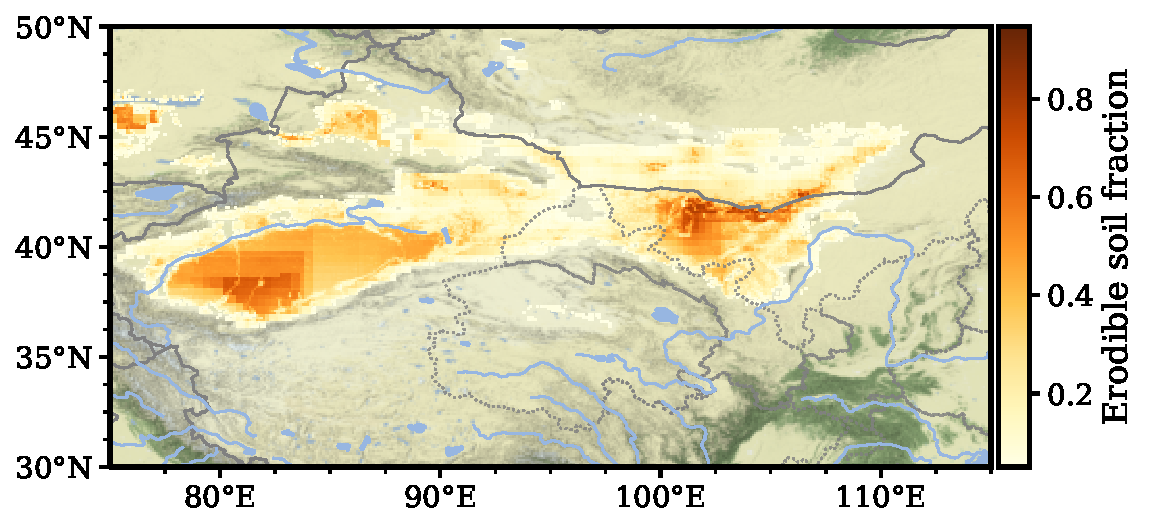
\includegraphics[width=\textwidth]{../figs/erodible_soil_fraction.pdf}
    \caption{The erodible soil fraction from FLEXDUST over the East Asia}
    \label{fig:erodible_soil_fraction_EA}
\end{figure}

The threshold friction velocity follow the idealised expression of \textcite{shao2000simple} in \Cref{eq:treshold_fric_vel}, and is determined by the \SI{75}{\micro\metre} particles. 
For regions with clay and silt present, but no sand, \SI{10}{\micro\metre} 
particles are set to determine the threshold friction velocity. The clay and 
silt fractions can either be obtained from ISRIC 250m resolution Soil Grids dataset 
\parencite{soil-grid_ref}, or using the default Global soil Data \cite{task2014global} dataset. 
The effect of soil moisture on the threshold friction velocity is parametrized according to \textcite{fecan1998parametrization}:
\begin{equation}
    \begin{cases}
    \frac{u_{*tw}}{u_{*t}}=1, & \text{if } w < w' \\
    \frac{u_{*tw}}{u_{*t}}=\sqrt{1+1.21(w-w')^{0.68}}, & w \geq w'
    \end{cases}
\end{equation}
Where $w$ is the volumetric water content of the soil (\%). If the soil moisture exceeds $w'$, the capillary 
forces will start affecting the threshold friction velocity. Here $w'$ is given by \Cref{eq:moisture_clay} 
and depends on the clay content $c$ (\%).   
\begin{equation} \label{eq:moisture_clay}
    w' = 0.17c + 0.0014c^2
\end{equation}
The soil moisture content is retrieved from the ECWMF input fields.
Furthermore, if the surface is covered by snow, dust emissions are assumed to be inhibited. 
Snow cover is available from the ECWMF input fields. 
\par In partly vegetated areas, non-erodible surface elements would increase the surface 
roughness affecting the dust emissions. In FLEXDUST, the drag partition to non-erodible 
surface elements for partly vegetated areas are accounted for following the description in 
\textcite{zender2003mineral}, by scaling the mobilisation threshold by $f_d$ according to \Cref{eq:drag_partition}:
\begin{equation}\label{eq:drag_partition}
    f_d = \left[1 - \frac{\ln (z_{0m}/z_{0s})}{0.35\ln (0.1/z_{0s})^{0.8}}\right]^{-1}
\end{equation}
Here $z_{0m}$ is the roughness length of momentum transfer, and $z_{0s}$ is the smooth roughness length which 
describes the roughness of a bed of potentially erodible particles without any non-erodible elements. Wind tunnel 
experiments have shown that: 
\begin{equation}
    z_{0s} \approx D/30
\end{equation}
where $D$ is the particle diameter. In FLEXDUST it is assumed globally uniform values of  $z_{0m}=\SI{100.0}{\micro\metre}$ and $z_{0s}=\SI{33.3}{\micro\metre}$.

After the mobilisation threshold is calculated,  the dust emissions flux is derived following the paremeterisation of the vertical dust flux as described in \textcite{MB95_dust_emission}: 
\begin{equation}
    F=c\alpha \frac{\rho u_{*}^3}{g}\left(1-\frac{u^2_{*t}}{u^2_*}\right)\left(1+ \frac{u_{*t}}{u_*}\right)
\end{equation}
where $u_*$ is the friction velocity, c is a constant scaling factor ($4.8\cdot 10^{-4}$) and $\alpha$ is the sand blasting efficiency:
\begin{equation}\label{eq:sand_blasing_eff}
    \alpha = 100\exp{(13.4f_{clay}-6)\ln 10}
\end{equation}
\Cref{eq:sand_blasing_eff} is only valid for clay fraction $\leq$ 0.2, so if the clay fraction exceed 0.2, it is set to 0.2 \parencite{zender2003mineral}. 


The small dust particles (< \SI{20}{\micro\metre}) has a greater potential to experience long-range transport due to their smaller settling velocities. Since FLEXDUST was developed to study long-range dust transport, the emitted dust is assumed to have a volume size distribution varying between \SI{0.2}{\micro\metre} and \SI{18.2}{\micro\metre}. This size distribution is based on brittle fragmentation theory described in \textcite{kok_scaling_2011}. The log-normal volume size distribution is determined according to \Cref{eq:size_dist}. 

\begin{equation}\label{eq:size_dist}
    \frac{\text{d} V_d}{\text{d} \ln D_d} = \frac{D_d}{c_v}\left[1 + \text{erf}\left(\frac{\ln(D_d/\overline{D_s})}{\sqrt{2}\ln \sigma_s}\right)\right]\text{exp}\left[-\left(\frac{D_d}{\lambda}\right)^3\right]
\end{equation}
Where $c_v = \SI{12.62}{\micro\metre}$ is a normalisation constant, $\overline{D_s}=\SI{3.4}{\micro\metre}$ and $\sigma_s = 3.0$ is the median diameter and the geometric standard deviation respectively.  

\section{FLEXible PARTicle Dispersion Model: FLEXPART}
\par The dust transport and deposition is calculated by the \acrfull{flexpart}. FLEXPART is an offline \acrshort{lpdm} that has been applied to study the transport of a wide range of atmospheric tracers, e.g. mineral dust, black carbon and volcanic ash \parencite{flexdust_ref_2016,choi_investigation_2020, eckhardt2008estimation}. 
The version of FLEXPART used is 10.4 and includes the improved wet deposition scheme based on cloud information from the ECWMF input fields \parencite{flexpart_wetdep}. 
\par FLEXPART calculates trajectories for a large number of computational particles (from here on referred to as particles and not be confused with real dust particles) that move according to the wind-fields resolved in the meteorological forcing with parameterizations of the turbulent motions, subgrid-scale convection, and gravitational settling imposed on the trajectories. 
Each particle represents a dust-aerosol population with a log-normal mass size distribution with a specified density and mean particle diameter. 
In addition, ice nucleation efficiency,$IN_{eff}$, cloud condensation nuclei efficiency $CCN_{eff}$ and efficiency of below cloud scavenging by rain $C_{rain}$ and snow $C_{snow}$, can be assigned to the particle regulating the strength of the wet deposition in the model.   

FLEXPART can be either run forward in time from the source to the receptor or backwards from the receptor to the source. The main difference between forward and backward simulations lies in how the emission strength is constrained. 
In a forward simulation, the particles are released at the source. 
The emitted mass which the particles carry is defined before the particle release, directly yielding the concentration and deposition on a regular longitude-latitude grid at each time step.
However, in a backward simulation, the particle release happens at the receptor, and the emission strength is unknown. 
The purpose of the particles in a backward simulation is to probe for the possible source regions and establish the emission sensitivity, i.e. how sensitive the deposition at the receptor would be to a potential source element. 
The final output corresponds to a distribution of possible source areas at each time step.
The emission sensitivity is constructed such that when multiplied by the emission flux with units \si{\kg\per\cubic\metre\per\s} would produce a map of how much each source element is contributing to the concentration or deposition at the receptor.
In a backward simulation, concentration, wet and dry deposition must be obtained through separate simulations as the particle release is set up differently depending on the configuration.  
\subsection{FLEXPART: dry deposition}
In FLEXPART, the dry deposition is represented by a dry deposition velocity $v_d(z)$, and when multiplied with the concentration at a specified height yields the deposition flux. 
FLEXPART includes both a dry deposition scheme for particulate matter as well as gasses and is calculated based on a two-layer resistance model \parencite{Flexpart-2005_ref_paper}.

In backward mode, dry deposition is calculated at the start of the simulation by releasing the particles in a shallow layer close to the ground. This layer corresponds to the layer in which particles in forward mode would be subjected to dry deposition, and is by default is set to 30m. The "mass" of the particles are then scaled by the deposition velocity and tracked backwards in time as in regular backward simulation \parencite{eckhardt2017source}. 

\subsection{FLEXPART wet deposition}
The wet deposition scheme in FLEXPART was recently improved in \textcite{flexpart_wetdep} to take advantage of cloud information available from the ECWMF forcing. The wet deposition scheme in FLEXPART consists of two steps.
First, the particle's location in relation to the cloud is determined using the 3D specific \acrfull{ctwc}. Then based on the particle's location in relation to the cloud, the particle can either be subjected to nucleation scavenging inside the cloud or impaction scavenging below the cloud. If the particle is above the cloud, no scavenging can occur. 

In backward mode, the wet deposition is calculated at the time of the particle release. Since wet deposition can occur throughout the whole atmospheric column, the particles are released over the whole atmospheric column to check if any particles are subjected to wet deposition. FLEXPART then calculates the trajectories for wet deposited particles starting at the height where the particles were scavenged, and the remaining particles are terminated.    
\subsubsection{In cloud scavenging}
The in-cloud scavenging scheme in FLEXPART is only activated for particles residing within a precipitating cloud. Precipitation does not necessarily occur over the whole grid cell in the input data. Accordingly, FLEXPART uses an empirical relation to derive the fraction of a gridcell experiencing precipitation; see \textcite{Flexpart-2005_ref_paper} for details. The subgrid precipitating cloud water (PCW) is calculated according to: 
\begin{equation}
    PCW = CTWC\frac{F}{cc}
\end{equation}
Here cc is the surface cloud cover, and F is the precipitating fraction of the gridcell. 

The aerosol scavenging coefficient $\Lambda$ (\si{\per\s}) for in cloud scavenging is given by:
\begin{equation}
    \Lambda = F_{nuc}\left(I/PWC\right)ic_r
\end{equation}
Where $F_{nuc}$ is the nucleation efficiency, I is the precipitation intensity, which is derived from the accumulated precipitation during one time interval in the ECWMF input data, and $ic_r$ is the cloud water replenishment rate. However, $ic_r$ cannot be determined from the ECWMF input data and was determined based on testing in FLEXPART and is considered a tuning parameter in the model.   

In reality, $F_{nuc}$ depends on many different parameters such as aerosol size, chemical composition, temperature and cloud phase. 
A complete parameterization of $F_{nuc}$ in FLEXPART is currently not possible based on the limited information available in the input forcing. 
Still, FLEXPART can account for the fact that aerosols have different nucleation efficiency depending on whether they serve as cloud condensation nuclei (CCN) or ice nuclei (IN). 
% For insoluble aerosols like mineral dust $CCN_{eff}$ primarily depends on the particle size. By itself mineral dust is usually not a very efficient CCN. However, by weathering during transport, the mineral dust aerosols might acquire a coating of some soluble material, e.g. sulphate, increasing its potential to act as a CCN \textcite{Dust_aerosols_coating2001}.     

\subsubsection{Below cloud scavenging}
Dust aerosols residing below the cloud might be scavenged by falling raindrops or snowflakes, called impaction scavenging. 
In FLEXPART, the probability of an aerosol being scavenged by liquid droplets is parameterised according to \textcite{laakso2003ultrafine}. 
The removal of aerosols by falling snowflakes is parameterised in \acrshort{flexpart} according to \textcite{kyro2009snow}.
The efficiency of scavenging by falling rain and snow can be adjusted in the model by changing the $C_{rain}$ and $C_{snow}$ parameter.   


\section{Model Setup}\label{sec:Model_setup}
FLEXPART and FLEXDUST were run at a 3hourly temporal resolution, $0.1\degree \times 0.1\degree$ spatial resolution and driven by  ERA5 meteorological forcing data. 
As described in \Cref{chap:east_asia_dust} dust events are primarily occurring in spring. Therefore only the spring months from March until May were included in the simulations. The models were run over a 20 year period to provide insight on the inter-annual variation in the dust source regions of the \acrshort{clp}.   

FLEXPART was set up in backward mode, and to cover the 20 year period, several independent FLEXPART simulations were set up, each covering one month.   
To make it possible to multiply the emission sensitivity with the dust emission flux, FLEXPART has to be set up such that each particle release is kept separate in the output. 
Therefore, a new particle release was specified in the \verb|RELEASES| file for each forward time step. The length of the trajectory was limited to five days by specifying a time limit in the \verb|NAGECLASSES| file.
The FLEXPART output file generated then contains two temporal dimensions, one \verb|time| dimension going from the last date backwards to the start date of the simulation and the \verb|pointspec| dimension that represents the forward time dimension. 
To allow for all the backward trajectories to complete, the last release have to happened five days after the starting date of the simulation.   
The particle release is specified at 3rd hourly intervals. The number of computational particles released in each release is 50000 particles and 200000 particles for dry and wet deposition simulations. 
More particles are released in the wet deposition due to how the particle release is setup and to ensure a
statically robust result.

\begin{figure}[htpb]
    \centering
    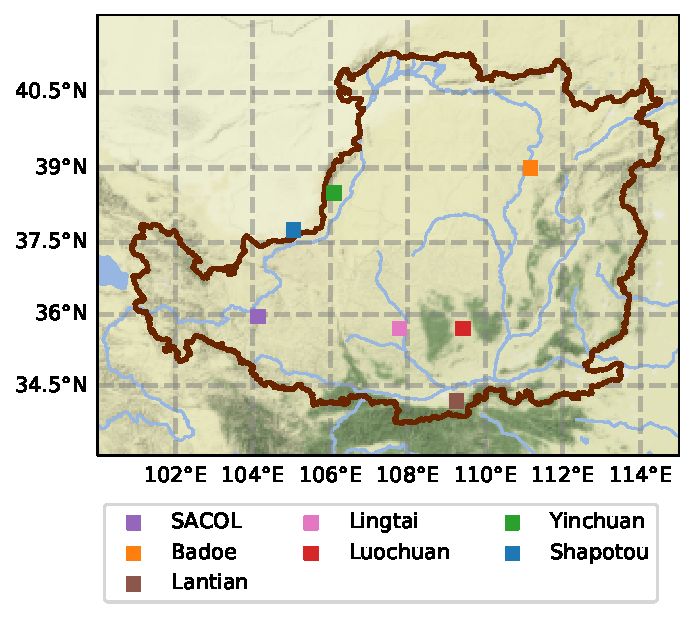
\includegraphics[width=0.7\textwidth]{texfiles/figs/map_loess.pdf}
    \caption{Map of the receptor points, for the deposition and source contribution is calculated}
    \label{fig:maps_clp_location}
\end{figure}

To be able to provide insight into the spatial variation in the dust source contribution to the \acrshort{clp}, seven well known Loess sites distributed across the \acrshort{clp} were selected as receptor points in FLEXPART  (\Cref{fig:maps_clp_location}), namely: SACOL, Shapotou and Yinchuan in the north west, Lingtai, Luochuan and Lantian in the south east and Badoe in the north east. 
The exact coordinates of the receptor locations are listed in \Cref{tab:coordinates_clp}. 

\begin{table}[htpb]
\caption{FLEXPART species parameters for "clay" and "silt" particle size bin}
\label{tab:particle_params}'
\centering
% \resizebox{\textwidth}{!}{%
\begin{tabular}{@{}lll@{}}
\toprule
 & Clay  & Silt \\ \midrule
\verb|PCRAIN_AERO| & 1.00  & 1.00 \\
\verb|PCSNOW_AERO| & 1.00  &  1.00 \\
\verb|PCC_AERO| & 0.45 \parencite{flexdust_ref_2016}   &  0.9\parencite{flexdust_ref_2016} \\
\verb|PIN_AERO| & 0.10 \parencite{flexdust_ref_2016} & 0.1 \parencite{flexdust_ref_2016} \\
\verb|PDENSITY| & \SI{2500.0}{\kg\per\cubic\metre}    & \SI{2500.0}{\kg\per\cubic\metre} \\
\verb|PDQUER| & \SI{2.057E-6}{\metre}    &  \SI{17.32E-6}{\metre}   \\
\verb|PDSIGMA| & 1.21   &  1.15    \\ \bottomrule
\end{tabular}%
% }
\end{table}

Moreover, two particles size bins, \SI{1.7}{\micro\metre}-\SI{2.5}{\micro\metre} representing clay particles and  \SI{15}{\micro\metre}-\SI{20}{\micro\metre} size bin representing silt sized particles were included in the FLEXPART simulations . 
The two particle size-bins did not only differ in their size, but they also had different assumptions on the $CCN_{eff}$ and $IN_{eff}$. 
The parameters for the two particle species are listed in \Cref{tab:particle_params}. 
This is a purely hypothetical size distribution. The coarse resolution of the size distribution was a trade-off to allow running multiple years and keep the computational demand reasonable.  

All in all, this added up to a total of 1680 individual FLEXPART simulations.
However, given that all the FLEXPART simulations are independent of each other, it was easy to take advantage of the large number of CPUs available on Saga.  
To help set up all the FLEXPART simulations, a python script\footnote{https://github.com/Ovewh/FLEXPART-script} was developed. 
FLEXDUST is much less demanding, and the whole 20-year simulation was done in a matter of a few hours on the supercomputer. 

\subsection{Model sensitivity experiments}
Sensitivity experiments are a crucial part of any modelling study. The aim of a sensitivity analysis is to quantify the impact of possible errors and differences in the input data on the predicted model output. Four sensitivity experiments were conducted, investigating the impact of (1) different forcing data, (2) varying particle density, (3) choice of soil texture data and (4) and below cloud scavenging. All the sensitivity experiments were done for 2019 except the forcing experiment done for 2015. Except for the parameters listed in \Cref{tab:sensitivity_exp} all other parameters are equal to the main model setup described previously. 

% The reason for testing the model with different forcing data is to examine how sensitive the results are to the choice of input data. The two forcing dataset compared in the sensitivity analysis is the latest generation of \acrshort{ecwmf} reanalysis, ERA5 against the previous generation of reanalysis ERA-Interim. This analysis would allow to whether using a the new higher resolution ERA5 as input data improves the representation of dust in the models. Moreover, if the difference between the two forcing dataset can reasonably explain based on there known differences, it means that  
\begin{table}[htpb]\label{tab:sensitivity_exp}
\caption{The model sensitivity experiments that have been performed}
\centering

\resizebox{\textwidth}{!}{%
\begin{tabular}{@{}lllll@{}}
\toprule
 Sensitivity experiment & Soil map  & Forcing & Below cloud scavenging & Particle density \\ \midrule
 Model forcing & ISRIC  & ERA-Interim & Yes & \SI{2500}{\kg\per\cubic\cm}  \\
 Particle density & ISRIC & ERA5  & Yes & \SI{2200}{\kg\per\cubic\cm}-\SI{2800}{\kg\per\cubic\cm}  \\
 Soil texture & Default & ERA5 & Yes & \SI{2500}{\kg\per\cubic\cm}   \\
 Cloud scavenging& ISRIC  & ERA5 & No & \SI{2500}{\kg\per\cubic\cm} \\ \bottomrule

\end{tabular}%
}
\end{table}

\section{Analysis Tools}

The analysis and post-processing of the model output are achieved using a handful of python libraries. Plotting and data visualisation:  \verb|matplotlib|, \verb|seaborn|, \verb|cartopy|. Data analysis and data processing: \verb|xarray|, \verb|numpy|, \verb|scikit-learn|, \verb|pandas|, \verb|dask|, \verb|snakemake| and \verb|jupyter|. The full anaconda environment listing the specific version of the packages are available on my GitHub. In addition, several python scripts were developed to facilitate the analysis and processing of the model output, and this is also available on my GitHub, or everything can be downloaded as a zip-file here \textbf{Link repo}. 

\subsection{Post-processing of model output}
The FLEXPART and FLEXDUST output fields have to be matched in order to calculate the source contribution. However, there is currently no software freely available that can match output from a backward simulation with an emission inventory. Therefore considerable effort had to be spent towards developing a code that could combine the FLEXPART and FLEXDUST output. First, the shape of the FLEXPART output data was changed into a format that would be easy to match with FLEXDUST. This was achieved by defining a new backwards time dimension with a length equal to maximum particle age (in this case, 5 days). Then set the \verb|pointspec| dimension was set as the main time dimension. This format is also a much more efficient way of storing the output from backward simulations. The original output format would only contain zeros after the maximum age was exceeded. When the output was converted to the new format, it was straightforward to match the FLEXDUST emission inventories with the FLEXPART emission sensitivity. 

When the FLEXPART and FLEXDUST output had been combined, emitted dust was assumed to have the following size distribution \textbf{some table}, the source contribution was then scaled by the fraction of the size distribution corresponding ...  

\subsection{FLEXPART trajectory analysis}
In addition to emission sensitivity, FLEXPART can output the centroid position of the particle cloud and cluster the particles into a specified number of cluster groups at each output interval. 
However, the clusters produced by FLEXPART are not very informative due to the clustering only being based on the position of the particles at the output time and does not consider which cluster it was previously assigned to.
The original idea was to the centroid trajectories of every particle release are re-clustered using the procedure described by \textcite{dorling1992cluster}.
This procedure is described in more detail in Appendix \labelcref{chap:trajec_analysis}. However this did not work out in the end for two reasons, (1) the challenge of defining an appropriate distance matrix and (2) in the cluster centriod many of the interesting features were already smoothed out. The code developed for reading the trajectory files and the doing the re-clustering can be accessed on GitHub \footnote{\url{https://github.com/Ovewh/flexpart_cluster}}. 

However I still wanted to take advantage of the trajectory information provided in FLEXPART. The alternative solution was then to do a clever selection of trajectories of only dust loading trajectories and then do a weighted average based on the amount of dust these trajectories carried.  

\subsection{Composite analysis}

Composite analysis is a useful method for identifying climatic features that are difficult to observe in its totally. A composite analysis involve collecting a number of cases of given situation, e.g. years with strong deposition, and create an average representation of meteorological conditions in that given situation, e.g. surface winds during strong deposition years. The to further magnify the changes one could subtract the cases where this particular situation is weak to produce composite anomalies.      





\begin{table}[]
    \caption{Caption}
    \label{tab:my_label}
    \centering
    \begin{tabular}{@{}ll@{}} 
    \toprule
         &  \\ \midrule
         
         & 
    \end{tabular}

\end{table}